\section{V13}
\subsection{Allgemeiner Ablauf von Exceptions und Interrupts}
\begin{minipage}{0.4\linewidth}
Interrupts werden in der Regel von der umgebenen Peripherie oder externen Input-Pins generiert und als Ereigniss der CPU-Infrastruktur signalisiert, welche dann eine Handler-Routine einschalten.\\
\textbf{Siehe} \nameref{Exceptions}
\end{minipage}
\begin{minipage}{0.6\linewidth}
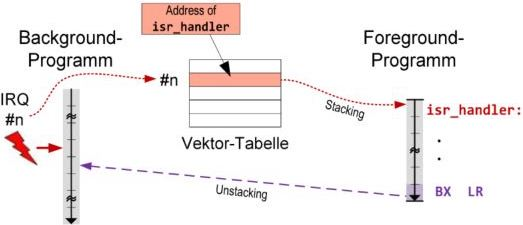
\includegraphics[width=\linewidth]{images/interruptablauf} 
\end{minipage}
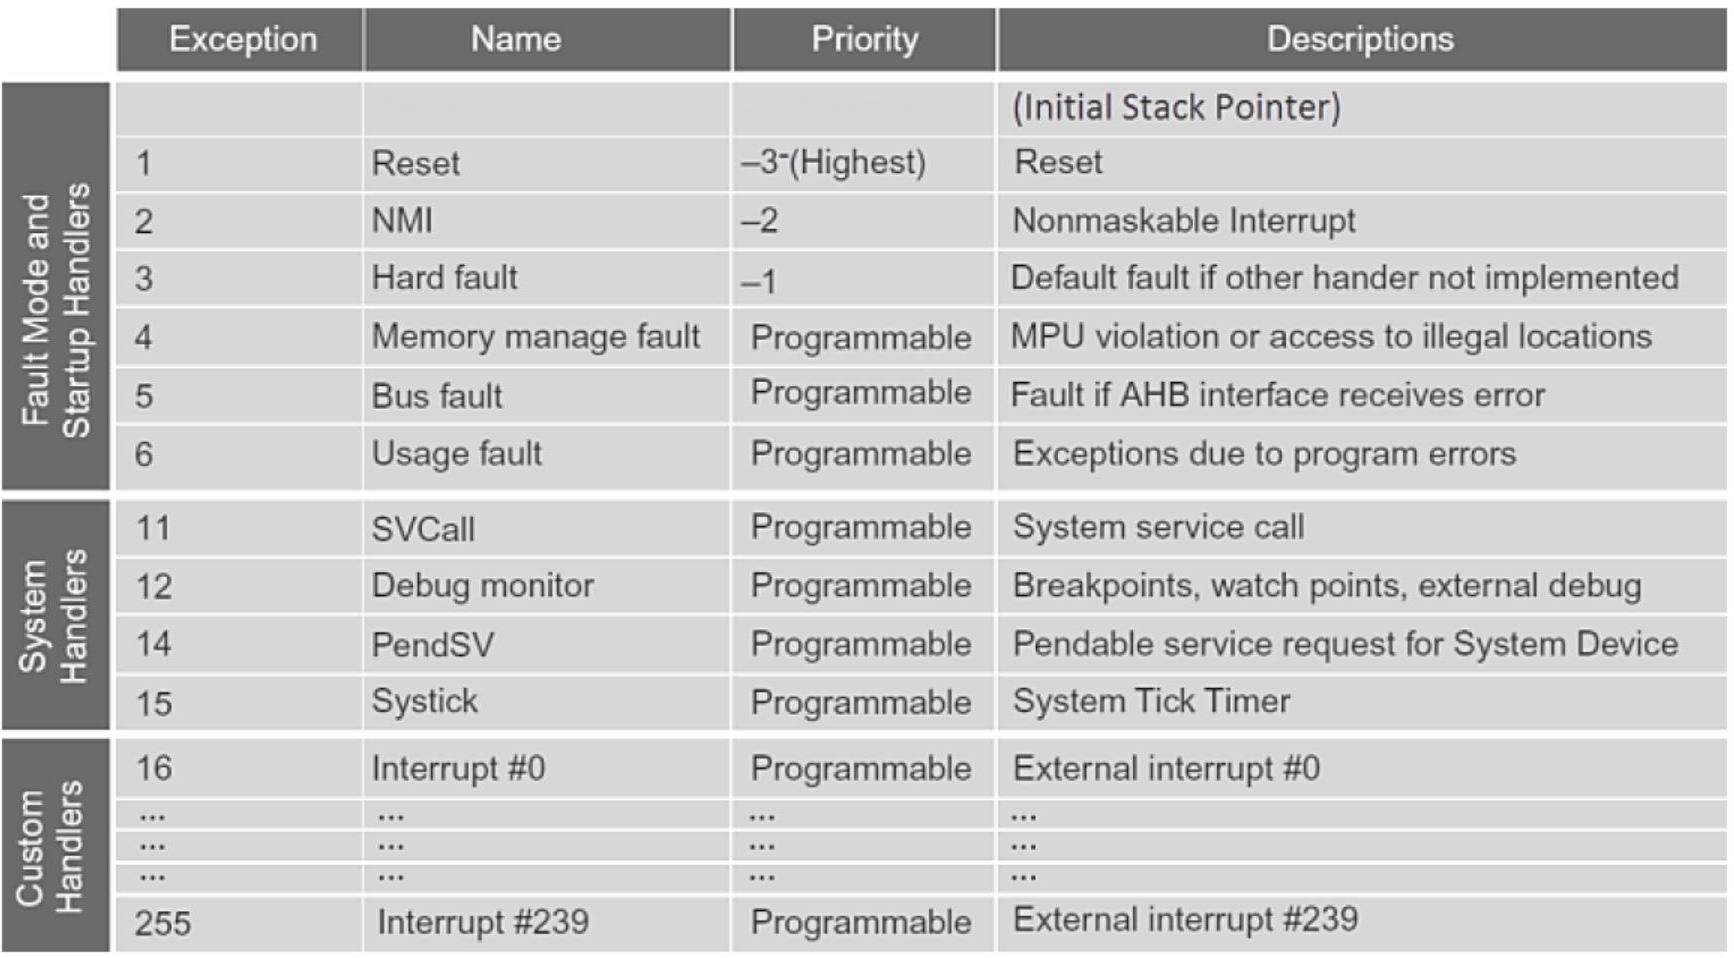
\includegraphics[width=0.8\linewidth]{images/NVICExcp1} 